\problemname{Grottflykt}
Av okänd anledning håller du på att utforska en grotta och har råkat väcka en arg björn.
Björnen är större och snabbare än du, så din enda chans är att överlista den för att ta dig ut.
Grottan kan representeras som ett rektangulärt bräde bestående av väggar och en utgång.
Du och björnen kan förflytta er i riktningarna upp, ner, höger eller vänster, men kan inte gå igenom väggar.

Varje gång du tagit ett steg, och inte kommit fram till utgången, så kommer björnen svara genom att flytta
högst $2$ steg i ett försök att ta sig så nära dig som möjligt. Om ni någon gång befinner er på samma ruta så är du förlorad.
Som tur är så är björnen inte helt medveten om väggar, och använder sig därför av en korkad algoritm för att flytta sig.

Det första björnen gör är att flytta sig mot dig i horisontell riktning. Detta gör den tills den fått slut på steg,
nått en vägg eller befinner sig i samma kolumn som du. Efter det gör den samma sak i vertikal riktning,
tills den fått slut på steg, nått en vägg eller befinner sig i samma rad som du. Det är alltså möjligt att björnen
förflyttar sig $0$, $1$ eller $2$ steg beroende på var du befinner dig och var det finns väggar.

Givet utseendet på grottan är det din uppgift att skriva ett program som hittar en sekvens av förflyttningar som låter dig fly grottan utan att bli fångad.

\begin{figure}[ht!]
\centering
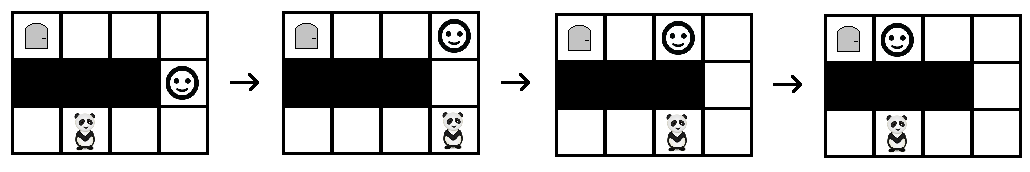
\includegraphics[width=\textwidth]{grottflykt.png}
\caption{En illustration av det första exemplet}
\label{overflow}
\end{figure}

\section*{Indata}
På första raden står två heltal $w$ och $h$ ($ 3 \leq w*h \leq 64$), grottans bredd och höjd.

Sedan följer $h$ rader med $w$ tecken var, en beskrivning av grottan. En vägg beskrivs med ``\#'', din startposition med ``S'',
utgången med ``U'' och björnen med ``B''. Det är garanterat att varje testfall går att lösa. 

\section*{Utdata}
Skriv ut en rad med en sträng bestående av tecken ``U'' för upp, ``N'' för ner, ``H'' för höger och ``V'' för vänster,
stegen du ska ta för att fly grottan. Ett svar som leder in i en vägg någon gång på vägen kommer inte godkännas.
Det är alltså inte möjligt att stå still en omgång genom att gå mot en vägg.

\noindent
\begin{tabular}{| l | l | p{12cm} |}
  \hline
  Grupp & Poängvärde & Gränser \\ \hline
  $1$    & $20$        & $h=1$ \\ \hline 
  $2$    & $30$        & $w*h \leq 25$ \\ \hline 
  $3$    & $50$        & Inga ytterligare begränsingar. \\ \hline 
\end{tabular}
